\documentclass[a4paper,12pt]{article}

% Packages
\usepackage{tikz}
\usepackage{circuitikz}
\usepackage{karnaugh-map}
\usepackage[margin=1in]{geometry}
\usepackage{amsmath}
\usepackage{graphicx}
\usepackage{float}
\usepackage{booktabs}
\usepackage{hyperref}

\title{Experiment:0 to 99 Synchronous Up/Down Counter using JK Flip-Flops}
\author{EE24BTECH11001 - Aditya Tripathy, EE24BTECH11018 - Durgi Swaraj Sharma}
\date{}

\begin{document}

\maketitle

\section*{Aim}
To design and implement a 0 to 99 synchronous up/down counter using JK flip-flops configured as T flip-flops.

\section*{Apparatus}
\begin{itemize}
  \item IC 7476 (JK Flip-Flop)
  \item IC 7411 (AND gates)
  \item IC 7432 (OR gates)
  \item IC 7447 (BCD Decoder)
  \item 7 Segment Displays
  \item Push buttons for UP and DOWN counting
  \item Breadboard and connecting wires
  \item Arduino UNO R3
\end{itemize}

\section*{Theory}
A MOD-10 counter goes through 10 states (0000 to 1001) before resetting to 0000. JK flip-flops can be configured as T flip-flops by connecting both J and K inputs together.

Each T flip-flop toggles on receiving a high (1) on its T input. The T inputs are generated by combinational logic based on the current state and the count direction (UP or DOWN).

The UP and DOWN signals are ANDed with the toggle logic of each flip-flop, and then both outputs are ORed to produce the final T input for each flip-flop.


\section*{Circuit Picture}
\begin{figure}[H]
  \centering
  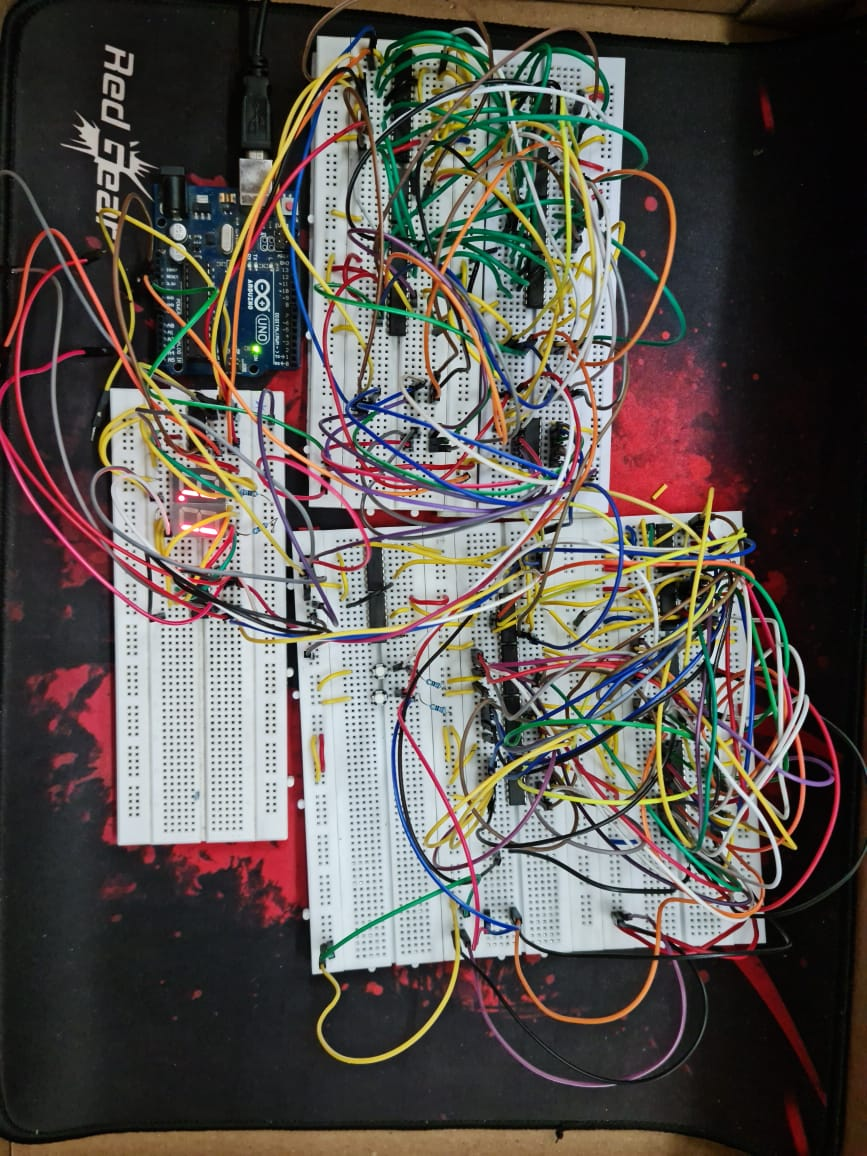
\includegraphics[width=0.5\textwidth]{circuit_picture.jpeg} % Replace with actual picture
  \caption{Actual implementation of the counter on breadboard}
\end{figure}
\begin{figure}[H]
  \centering
  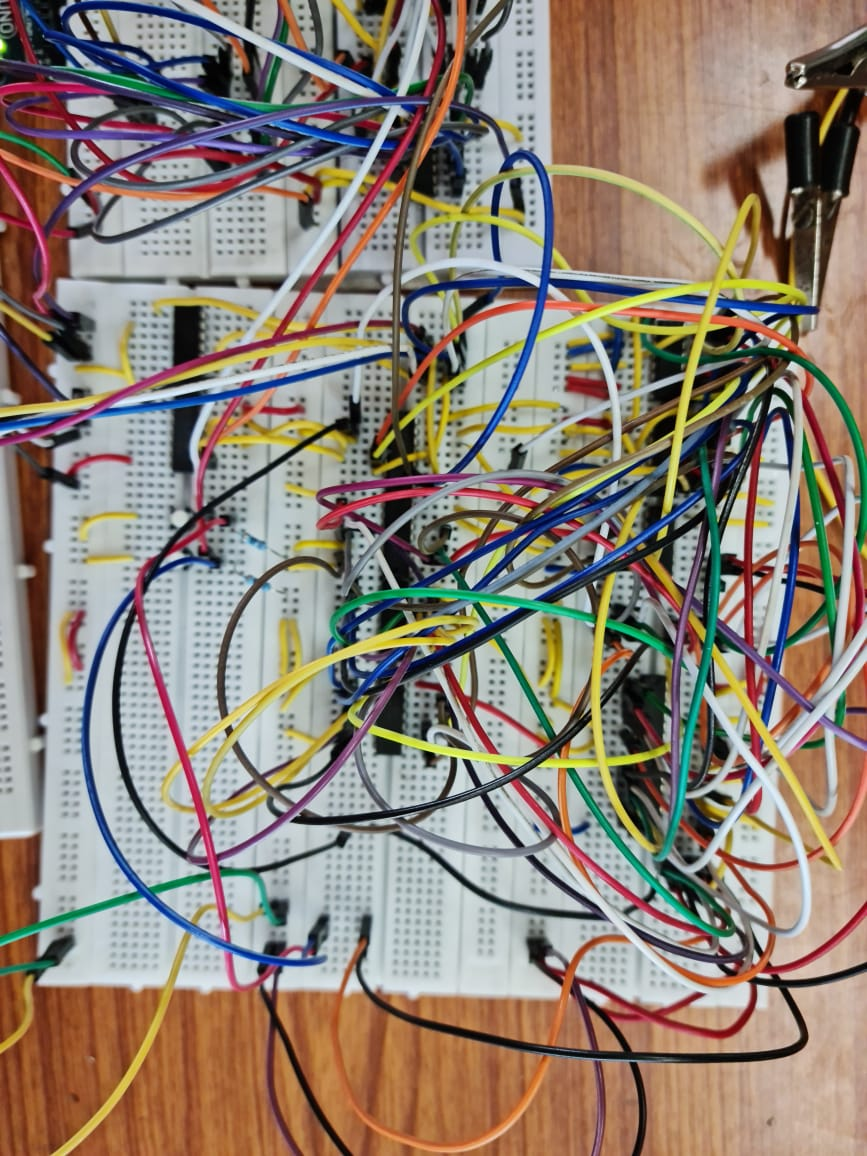
\includegraphics[width=0.5\textwidth]{circuit_picture_2.jpeg} % Replace with actual picture
\end{figure}
\begin{figure}[H]
  \centering
  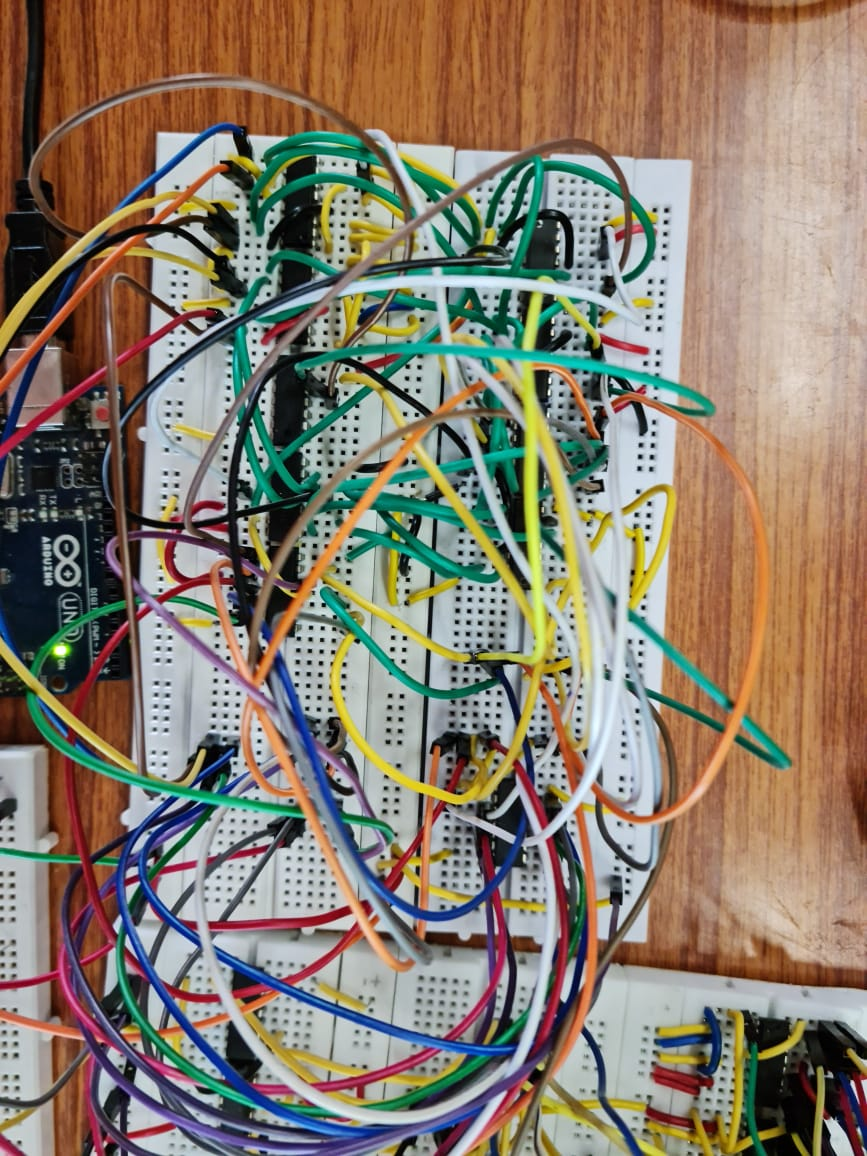
\includegraphics[width=0.5\textwidth]{circuit_picture_3.jpeg} % Replace with actual picture
\end{figure}
\begin{figure}[H]
  \centering
  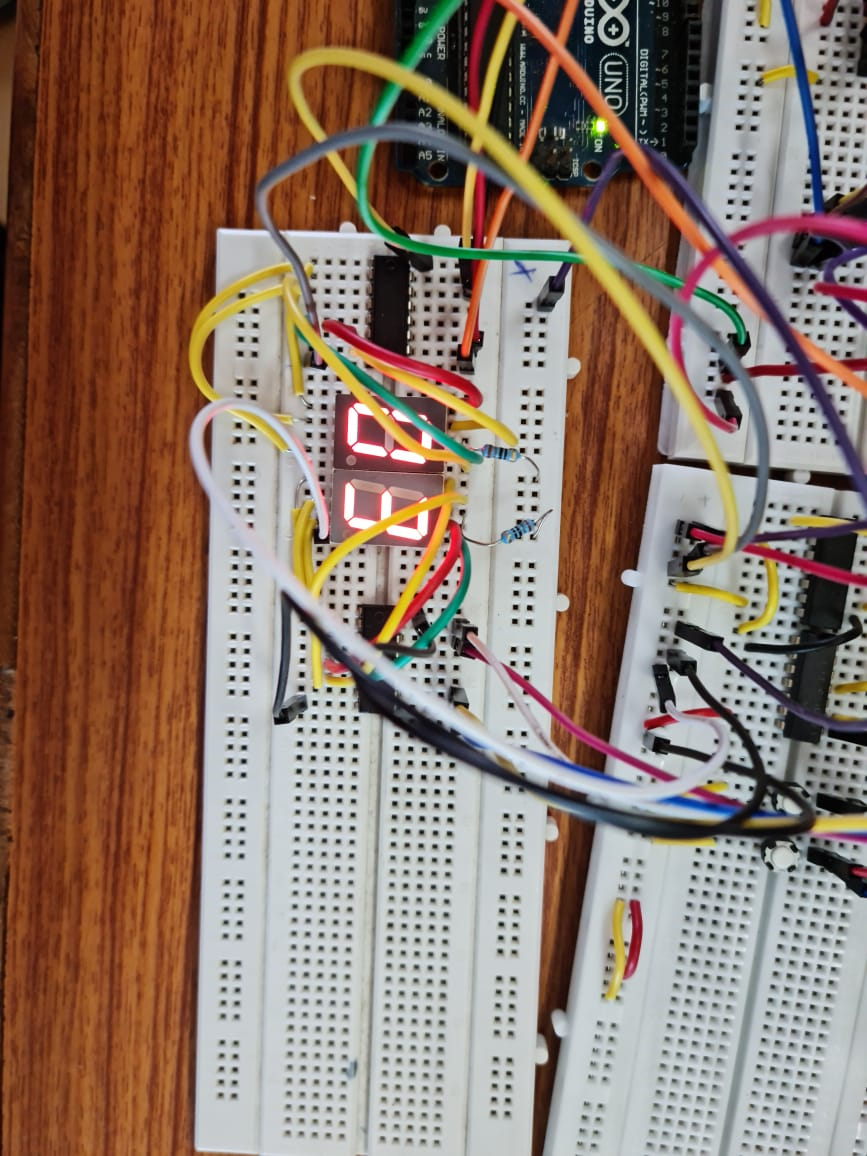
\includegraphics[width=0.5\textwidth]{circuit_picture_4.jpeg} % Replace with actual picture
\end{figure}
\section*{State Transition Table (Up Count)}
\begin{center}
\begin{tabular}{ccccccc}
\toprule
Present State & Next State (Up) & T\textsubscript{3}$^\text{up}$ & T\textsubscript{2}$^\text{up}$ & T\textsubscript{1}$^\text{up}$ & T\textsubscript{0}$^\text{up}$ \\
\midrule
0000 (0) & 0001 (1) & 0 & 0 & 0 & 1 \\
0001 (1) & 0010 (2) & 0 & 0 & 1 & 1 \\
0010 (2) & 0011 (3) & 0 & 0 & 0 & 1 \\
0011 (3) & 0100 (4) & 0 & 1 & 1 & 1 \\
0100 (4) & 0101 (5) & 0 & 0 & 0 & 1 \\
0101 (5) & 0110 (6) & 0 & 0 & 1 & 1 \\
0110 (6) & 0111 (7) & 0 & 0 & 0 & 1 \\
0111 (7) & 1000 (8) & 1 & 1 & 1 & 1 \\
1000 (8) & 1001 (9) & 0 & 0 & 0 & 1 \\
1001 (9) & 0000 (0) & 1 & 0 & 0 & 1 \\
\bottomrule
\end{tabular}
\end{center}

\section*{State Transition Table (Down Count)}
\begin{center}
\begin{tabular}{ccccccc}
\toprule
Present State & Next State (Down) & T\textsubscript{3}$^\text{down}$ & T\textsubscript{2}$^\text{down}$ & T\textsubscript{1}$^\text{down}$ & T\textsubscript{0}$^\text{down}$ \\
\midrule
0000 (0) & 1001 (9) & 1 & 0 & 0 & 1 \\
0001 (1) & 0000 (0) & 0 & 0 & 0 & 1 \\
0010 (2) & 0001 (1) & 0 & 0 & 1 & 1 \\
0011 (3) & 0010 (2) & 0 & 0 & 0 & 1 \\
0100 (4) & 0011 (3) & 0 & 1 & 1 & 1 \\
0101 (5) & 0100 (4) & 0 & 0 & 0 & 1 \\
0110 (6) & 0101 (5) & 0 & 0 & 1 & 1 \\
0111 (7) & 0110 (6) & 0 & 0 & 0 & 1 \\
1000 (8) & 0111 (7) & 1 & 1 & 1 & 1 \\
1001 (9) & 1000 (8) & 0 & 0 & 0 & 1 \\
\bottomrule
\end{tabular}
\end{center}

\section*{Karnaugh Maps for T Flip-Flops}

\subsection*{Up Counter T Flip-Flops}
\textbf{For \(T_0\):}  
Since \(T_0 = 1\) for all cases, no Karnaugh map is required.

\vspace{0.5cm}
\textbf{For \(T_1\):}
\begin{center}
\begin{karnaugh-map}[4][4][1][$Q_1Q_0$][$Q_3Q_2$]
\manualterms{0,1,0,1,0,1,0,1,0,0,X,X,X,X,X,X}
\end{karnaugh-map}
\end{center}
Thus, 
\[
T_1 = \overline{Q_3}\,Q_0.
\]

\vspace{0.3cm}
\textbf{For \(T_2\):}
\begin{center}
\begin{karnaugh-map}[4][4][1][$Q_1Q_0$][$Q_3Q_2$]
\manualterms{0,0,0,1,0,0,0,1,0,0,X,X,X,X,X,X}
\end{karnaugh-map}
\end{center}
Thus, 
\[
T_2 = Q_1\,Q_0.
\]

\vspace{0.5cm}
\textbf{For \(T_3\):}
\begin{center}
\begin{karnaugh-map}[4][4][1][$Q_1Q_0$][$Q_3Q_2$]
\manualterms{0,0,0,0,0,0,0,1,0,1,X,X,X,X,X,X}
\end{karnaugh-map}
\end{center}
Thus, 
\[
T_3 = Q_2\,Q_1\,Q_0 + Q_3\,Q_0.
\]

\subsection*{Down Counter T Flip-Flops}
\textbf{For \(T_0\):}  
Again, \(T_0 = 1\) for all cases.

\vspace{0.5cm}
\textbf{For \(T_1\):}
\begin{center}
\begin{karnaugh-map}[4][4][1][$Q_1Q_0$][$Q_3Q_2$]
\manualterms{0,0,1,0,1,0,1,0,1,0,X,X,X,X,X,X}
\end{karnaugh-map}
\end{center}
Thus,
\[
T_1 = Q_1\,\overline{Q_0} + Q_2\,\overline{Q_1}\overline{Q_0} + Q_3\,\overline{Q_1}\,\overline{Q_0}.
\]

\vspace{0.5cm}
\textbf{For \(T_2\):}
\begin{center}
\begin{karnaugh-map}[4][4][1][$Q_1Q_0$][$Q_3Q_2$]
\manualterms{0,0,0,0,1,0,0,0,1,0,X,X,X,X,X,X}
\end{karnaugh-map}
\end{center}
Thus,
\[
T_2 = Q_2\,\overline{Q_1}\,\overline{Q_0} + Q_3\,\overline{Q_1}\,\overline{Q_0}.
\]

\vspace{0.5cm}
\textbf{For \(T_3\):}
\begin{center}
\begin{karnaugh-map}[4][4][1][$Q_1Q_0$][$Q_3Q_2$]
\manualterms{1,0,0,0,0,0,0,0,1,0,X,X,X,X,X,X}
\end{karnaugh-map}
\end{center}
Thus,
\[
T_3 = \overline{Q_2}\,\overline{Q_1}\,\overline{Q_0}
\]

The circuit is easier to build if we take $T = \overline{Q_1}\,\overline{Q_0}$ then:
\begin{enumerate}
    \item $T_0 = 1$
    \item $T_1 = Q_1\,\overline{Q_0} = T_2$
    \item $T_2 = (Q_1 + Q_2)T$
    \item $T_3 = \overline{Q_2}\,T$
\end{enumerate}
due to the type of ICs we have (3 input AND gates and 2 input OR gates)
\section*{Procedure}
\subsection*{One's Digit}
For each flip flop, the T pin should either receive incrementing combinational logic or decrementing logic based on whether the "up button" is pressed or the "down" button is pressed. This is achieved as shown the following diagram
\begin{figure}[!ht]
\centering
\resizebox{0.8\textwidth}{!}{%
\begin{circuitikz}
\tikzstyle{every node}=[font=\normalsize]
\draw (5,17.5) to[short] (5.75,17.5);
\draw (5,17) to[short] (5.75,17);
\draw (5.75,17.5) node[ieeestd and port, anchor=in 1, scale=0.89](port){} (port.out) to[short] (8.25,17.25);
\draw (5,14.5) to[short] (5.75,14.5);
\draw (5,14) to[short] (5.75,14);
\draw (5.75,14.5) node[ieeestd and port, anchor=in 1, scale=0.89](port){} (port.out) to[short] (8.25,14.25);
\draw (9.5,16) to[short] (9.75,16);
\draw (9.5,15.5) to[short] (9.75,15.5);
\draw (9.75,16) node[ieeestd or port, anchor=in 1, scale=0.89](port){} (port.out) to[short] (11.5,15.75);
\draw (8.25,17.25) to[short] (8.25,16);
\draw (9.5,16) to[short] (8.25,16);
\draw (8.25,14.25) to[short] (8.25,15.5);
\draw (9.5,15.5) to[short] (8.25,15.5);
\draw (5,17.5) to[short] (5,19.25);
\draw (5,19.25) to[short] (3.5,19.25);
\draw (5,14) to[short] (5,12.5);
\draw (5,12.5) to[short] (3.75,12.5);
\draw  (0,18) rectangle (4.25,16.25);
\draw  (0,15.25) rectangle (4.25,13);
\draw [short] (5.25,17) -- (4.25,17);
\draw [short] (5,14.5) -- (4.25,14.5);
\node [font=\normalsize] at (2.25,12.5) {down count signal};
\node [font=\normalsize] at (2.25,14.25) {decrement logic};
\node [font=\normalsize] at (2.25,17.25) {increment logic};
\node [font=\normalsize] at (2.25,19.25) {up count signal};
\node [font=\LARGE] at (12.5,15.75) {$T_i$};
\end{circuitikz}
}%

\label{One's Place multiplexing}
\end{figure}
From this diagram it is clear that when the up count button is pressed, then the signal passed to the T pin of the flip flop will be the result of the incrementing synchronous counter k-map results, and likewise for when the down count button is pressed.
\subsection*{Ten's Digit}
For the ten's digit, we should increment tens place automatically (without any additional button presses) when the ones digit is 9 (1001 in binary). Likewise we will decrement the ten's place when one's place is zero (0000 in binary). The process is made clear by the following diagrams:
\begin{figure}[H]
\centering
\resizebox{0.5\textwidth}{!}{%
\begin{circuitikz}
\tikzstyle{every node}=[font=\normalsize]
\draw (5,17.5) to[short] (5.75,17.5);
\draw (5,17) to[short] (5.75,17);
\draw (5.75,17.5) node[ieeestd and port, anchor=in 1, scale=0.89](port){} (port.out) to[short] (8.25,17.25);
\draw (port.left) to[short] (5,17.25);
\draw (5,14.5) to[short] (5.75,14.5);
\draw (5,14) to[short] (5.75,14);
\draw (5.75,14.5) node[ieeestd and port, anchor=in 1, scale=0.89](port){} (port.out) to[short] (8.25,14.25);
\draw (port.left) to[short] (5,14.25);
\draw (9.5,16) to[short] (9.75,16);
\draw (9.5,15.5) to[short] (9.75,15.5);
\draw (9.75,16) node[ieeestd or port, anchor=in 1, scale=0.89](port){} (port.out) to[short] (11.5,15.75);
\draw (8.25,17.25) to[short] (8.25,16);
\draw (9.5,16) to[short] (8.25,16);
\draw (8.25,14.25) to[short] (8.25,15.5);
\draw (9.5,15.5) to[short] (8.25,15.5);
\draw (5,17.5) to[short] (5,19.25);
\draw (5,19.25) to[short] (3.5,19.25);
\draw (5,14) to[short] (5,11.5);
\draw  (0,18) rectangle (4.25,16.25);
\draw  (0,15.25) rectangle (4.25,13);
\draw [short] (5.25,17) -- (4.25,17);
\draw [short] (5,14.5) -- (4.25,14.5);
\node [font=\normalsize] at (2.25,11.5) {down count signal};
\node [font=\normalsize] at (2.25,14.25) {decrement logic};
\node [font=\normalsize] at (2.25,17.25) {increment logic};
\node [font=\normalsize] at (2.25,19.25) {up count signal};
\node [font=\normalsize] at (12,15.75) {$T_3$};
\draw (5,14.25) to[short] (4.5,14.25);
\draw (4.5,14.25) to[short] (4.5,12.25);
\draw (5,11.5) to[short] (3.75,11.5);
\draw (4.5,12.25) to[short] (2.75,12.25);
\draw (5,17.25) to[short] (4.5,17.25);
\draw (4.5,17.25) to[short] (4.5,18.5);
\draw (4.5,18.5) to[short] (2.5,18.5);
\node [font=\normalsize] at (2,18.5) {$Q_3 ^{\text{one's}}$};
\node [font=\normalsize] at (2.25,12.25) {$\overline{Q_3^{\text{one's}}}$};
\end{circuitikz}
}%

\label{fig:my_label}
\end{figure}
\begin{figure}[H]
\centering
\resizebox{0.5\textwidth}{!}{%
\begin{circuitikz}
\tikzstyle{every node}=[font=\normalsize]
\draw (5,17.5) to[short] (5.75,17.5);
\draw (5,17) to[short] (5.75,17);
\draw (5.75,17.5) node[ieeestd and port, anchor=in 1, scale=0.89](port){} (port.out) to[short] (8.25,17.25);
\draw (port.left) to[short] (5,17.25);
\draw (5,14.5) to[short] (5.75,14.5);
\draw (5,14) to[short] (5.75,14);
\draw (5.75,14.5) node[ieeestd and port, anchor=in 1, scale=0.89](port){} (port.out) to[short] (8.25,14.25);
\draw (port.left) to[short] (5,14.25);
\draw (9.5,16) to[short] (9.75,16);
\draw (9.5,15.5) to[short] (9.75,15.5);
\draw (9.75,16) node[ieeestd or port, anchor=in 1, scale=0.89](port){} (port.out) to[short] (11.5,15.75);
\draw (8.25,17.25) to[short] (8.25,16);
\draw (9.5,16) to[short] (8.25,16);
\draw (8.25,14.25) to[short] (8.25,15.5);
\draw (9.5,15.5) to[short] (8.25,15.5);
\draw (5,17.5) to[short] (5,19.25);
\draw (5,19.25) to[short] (3.5,19.25);
\draw (5,14) to[short] (5,11.5);
\draw  (0,18) rectangle (4.25,16.25);
\draw  (0,15.25) rectangle (4.25,13);
\draw [short] (5.25,17) -- (4.25,17);
\draw [short] (5,14.5) -- (4.25,14.5);
\node [font=\normalsize] at (2.25,11.5) {down count signal};
\node [font=\normalsize] at (2.25,14.25) {decrement logic};
\node [font=\normalsize] at (2.25,17.25) {increment logic};
\node [font=\normalsize] at (2.25,19.25) {up count signal};
\node [font=\normalsize] at (12,15.75) {$T_2$};
\draw (5,14.25) to[short] (4.5,14.25);
\draw (4.5,14.25) to[short] (4.5,12.25);
\draw (5,11.5) to[short] (3.75,11.5);
\draw (4.5,12.25) to[short] (2.75,12.25);
\draw (5,17.25) to[short] (4.5,17.25);
\draw (4.5,17.25) to[short] (4.5,18.5);
\draw (4.5,18.5) to[short] (2.5,18.5);
\node [font=\normalsize] at (2,18.5) {$\overline{Q_2^{\text{one's}}}$};
\node [font=\normalsize] at (2.25,12.25) {$\overline{Q_2^{\text{one's}}}$};
\end{circuitikz}
}%

\label{fig:my_label}
\end{figure}
\begin{figure}[H]
\centering
\resizebox{0.5\textwidth}{!}{%
\begin{circuitikz}
\tikzstyle{every node}=[font=\normalsize]
\draw (5,17.5) to[short] (5.75,17.5);
\draw (5,17) to[short] (5.75,17);
\draw (5.75,17.5) node[ieeestd and port, anchor=in 1, scale=0.89](port){} (port.out) to[short] (8.25,17.25);
\draw (port.left) to[short] (5,17.25);
\draw (5,14.5) to[short] (5.75,14.5);
\draw (5,14) to[short] (5.75,14);
\draw (5.75,14.5) node[ieeestd and port, anchor=in 1, scale=0.89](port){} (port.out) to[short] (8.25,14.25);
\draw (port.left) to[short] (5,14.25);
\draw (9.5,16) to[short] (9.75,16);
\draw (9.5,15.5) to[short] (9.75,15.5);
\draw (9.75,16) node[ieeestd or port, anchor=in 1, scale=0.89](port){} (port.out) to[short] (11.5,15.75);
\draw (8.25,17.25) to[short] (8.25,16);
\draw (9.5,16) to[short] (8.25,16);
\draw (8.25,14.25) to[short] (8.25,15.5);
\draw (9.5,15.5) to[short] (8.25,15.5);
\draw (5,17.5) to[short] (5,19.25);
\draw (5,19.25) to[short] (3.5,19.25);
\draw (5,14) to[short] (5,11.5);
\draw  (0,18) rectangle (4.25,16.25);
\draw  (0,15.25) rectangle (4.25,13);
\draw [short] (5.25,17) -- (4.25,17);
\draw [short] (5,14.5) -- (4.25,14.5);
\node [font=\normalsize] at (2.25,11.5) {down count signal};
\node [font=\normalsize] at (2.25,14.25) {decrement logic};
\node [font=\normalsize] at (2.25,17.25) {increment logic};
\node [font=\normalsize] at (2.25,19.25) {up count signal};
\node [font=\normalsize] at (12,15.75) {$T_1$};
\draw (5,14.25) to[short] (4.5,14.25);
\draw (4.5,14.25) to[short] (4.5,12.25);
\draw (5,11.5) to[short] (3.75,11.5);
\draw (4.5,12.25) to[short] (2.75,12.25);
\draw (5,17.25) to[short] (4.5,17.25);
\draw (4.5,17.25) to[short] (4.5,18.5);
\draw (4.5,18.5) to[short] (2.5,18.5);
\node [font=\normalsize] at (2,18.5) {$\overline{Q_1^{\text{one's}}}$};
\node [font=\normalsize] at (2.25,12.25) {$\overline{Q_1^{\text{one's}}}$};
\end{circuitikz}
}%

\label{fig:my_label}
\end{figure}


\begin{figure}[H]
\centering
\resizebox{0.5\textwidth}{!}{%
\begin{circuitikz}
\tikzstyle{every node}=[font=\normalsize]
\draw (5,17.5) to[short] (5.75,17.5);
\draw (5,17) to[short] (5.75,17);
\draw (5.75,17.5) node[ieeestd and port, anchor=in 1, scale=0.89](port){} (port.out) to[short] (8.25,17.25);
\draw (port.left) to[short] (5,17.25);
\draw (5,14.5) to[short] (5.75,14.5);
\draw (5,14) to[short] (5.75,14);
\draw (5.75,14.5) node[ieeestd and port, anchor=in 1, scale=0.89](port){} (port.out) to[short] (8.25,14.25);
\draw (port.left) to[short] (5,14.25);
\draw (9.5,16) to[short] (9.75,16);
\draw (9.5,15.5) to[short] (9.75,15.5);
\draw (9.75,16) node[ieeestd or port, anchor=in 1, scale=0.89](port){} (port.out) to[short] (11.5,15.75);
\draw (8.25,17.25) to[short] (8.25,16);
\draw (9.5,16) to[short] (8.25,16);
\draw (8.25,14.25) to[short] (8.25,15.5);
\draw (9.5,15.5) to[short] (8.25,15.5);
\draw (5,17.5) to[short] (5,19.25);
\draw (5,19.25) to[short] (3.5,19.25);
\draw (5,14) to[short] (5,11.5);
\draw  (0,18) rectangle (4.25,16.25);
\draw  (0,15.25) rectangle (4.25,13);
\draw [short] (5.25,17) -- (4.25,17);
\draw [short] (5,14.5) -- (4.25,14.5);
\node [font=\normalsize] at (2.25,11.5) {down count signal};
\node [font=\normalsize] at (2.25,14.25) {decrement logic};
\node [font=\normalsize] at (2.25,17.25) {increment logic};
\node [font=\normalsize] at (2.25,19.25) {up count signal};
\node [font=\normalsize] at (12,15.75) {$T_0$};
\draw (5,14.25) to[short] (4.5,14.25);
\draw (4.5,14.25) to[short] (4.5,12.25);
\draw (5,11.5) to[short] (3.75,11.5);
\draw (4.5,12.25) to[short] (2.75,12.25);
\draw (5,17.25) to[short] (4.5,17.25);
\draw (4.5,17.25) to[short] (4.5,18.5);
\draw (4.5,18.5) to[short] (2.5,18.5);
\node [font=\normalsize] at (2,18.5) {$Q_0^{\text{one's}}$};
\node [font=\normalsize] at (2.25,12.25) {$\overline{Q_0^{\text{one's}}}$};
\end{circuitikz}
}%

\label{fig:my_label}
\end{figure}
Therefore we can see that we are passing the incrementing logic to the respective T pins of the flip flop when the ones place is 9 ( $Q_3^{\text{one's}} = 1, Q_2^{\text{one's}} = 0, Q_1^{\text{one's}} = 0, Q_0^{\text{one's}} = 1$) and we pass decrement logic when ones pace is zero ($Q_3^{\text{one's}} = Q_2^{\text{one's}} = Q_1^{\text{one's}} = Q_0^{\text{one's}} = 0$).

\section*{Circuit Diagram}
\subsection*{One's Digit}
\begin{figure}[!ht]
\centering
\resizebox{1\textwidth}{!}{%
\begin{circuitikz}
\tikzstyle{every node}=[font=\LARGE]
\draw  (5,15.75) rectangle (8.75,10.75);
\draw  (11.25,15.75) rectangle (15,10.75);
\draw  (17.5,15.75) rectangle (21.25,10.75);
\draw  (-1.25,15.75) rectangle (2.5,10.75);
\node [font=\LARGE] at (-0.5,15) {$T_0$};
\node [font=\LARGE] at (-0.5,11.25) {Clk};
\node [font=\LARGE] at (2,14.5) {$Q_0$};
\node [font=\LARGE] at (2,12) {$Q_0$};
\draw (1.5,12.5) to[short] (2.25,12.5);
\node [font=\LARGE] at (5.75,15) {$T_1$};
\node [font=\LARGE] at (8.25,14.5) {$Q_1$};
\node [font=\LARGE] at (8.25,12) {$Q_1$};
\draw (7.75,12.5) to[short] (8.5,12.5);
\node [font=\LARGE] at (5.75,11.25) {Clk};
\node [font=\LARGE] at (12,15) {$T_2$};
\node [font=\LARGE] at (14.5,14.5) {$Q_2$};
\node [font=\LARGE] at (14.5,12) {$Q_2$};
\draw (14,12.5) to[short] (14.75,12.5);
\node [font=\LARGE] at (12,11.25) {Clk};
\node [font=\LARGE] at (18.25,15) {$T_3$};
\node [font=\LARGE] at (20.75,14.5) {$Q_3$};
\node [font=\LARGE] at (20.75,12) {$Q_3$};
\draw (20.25,12.5) to[short] (21,12.5);
\node [font=\LARGE] at (18.25,11.25) {Clk};
\draw (-6.25,9.5) to[short] (-2.5,9.5);
\draw (-2.5,9.5) to[short] (-2.5,11.5);
\draw (-2.5,11.5) to[short] (-1.25,11.5);
\draw (-2.5,9.5) to[short] (3.75,9.5);
\draw (3.75,9.5) to[short] (3.75,11.5);
\draw (3.75,11.5) to[short] (5,11.5);
\draw (3.75,9.5) to[short] (10,9.5);
\draw (10,9.5) to[short] (10,11.5);
\draw (10,11.5) to[short] (11.25,11.5);
\draw (10,9.5) to[short] (16.25,9.5);
\draw (16.25,9.5) to[short] (16.25,11.5);
\draw (16.25,11.5) to[short] (17.5,11.5);
\draw (-1.25,15) to[short] (-2,15);
\draw (-2,15) to[battery1] (-2,16.5);
\draw (-2,16.5) to (-3,16.5) node[ground]{};
\draw (21.25,12) to[short] (22.5,12);
\draw (22.5,12) to[short] (23.25,12);
\draw (23.25,12) to[short] (23.25,16.5);
\draw (23.25,16.5) to[short] (7,16.5);
\draw (2.5,14.5) to[short] (3,14.5);
\draw (7,17) to[short] (6.75,17);
\draw (7,16.5) to[short] (6.75,16.5);
\draw (6.75,17) node[ieeestd and port, anchor=in 2, scale=0.89, rotate=180](port){} (port.out) to[short] (4.75,16.75);
\draw (3,14.5) to[short] (3,18);
\draw (3,18) to[short] (7,18);
\draw (7,18) to[short] (7,17);
\draw (4.75,16.75) to[short] (4.25,16.75);
\draw (4.25,16.75) to[short] (4.25,15);
\draw (4.25,15) to[short] (5,15);
\draw (8,18.25) to[short] (8.5,18.25);
\draw (8,17.75) to[short] (8.5,17.75);
\draw (8.5,18.25) node[ieeestd and port, anchor=in 1, scale=0.89](port){} (port.out) to[short] (10.75,18);
\draw (8.75,14.5) to[short] (9.25,14.5);
\draw (9.25,14.5) to[short] (9.25,16.75);
\draw (9.25,16.75) to[short] (8,16.75);
\draw (8,16.75) to[short] (8,17.75);
\draw (8,18.25) to[short] (7,18.25);
\draw (7,18.25) to[short] (7,17.75);
\draw (10.75,18) to[short] (10.75,15);
\draw (10.75,15) to[short] (11.25,15);
\draw (16.25,18.75) to[short] (16.5,18.75);
\draw (16.25,18.25) to[short] (16.5,18.25);
\draw (16.5,18.75) node[ieeestd or port, anchor=in 1, scale=0.89](port){} (port.out) to[short] (18.25,18.5);
\draw (13.25,19.5) to[short] (13.5,19.5);
\draw (13.25,19) to[short] (13.5,19);
\draw (13.5,19.5) node[ieeestd and port, anchor=in 1, scale=0.89](port){} (port.out) to[short] (15.25,19.25);
\draw (13.25,17.75) to[short] (13.5,17.75);
\draw (13.25,17.25) to[short] (13.5,17.25);
\draw (13.5,17.75) node[ieeestd and port, anchor=in 1, scale=0.89](port){} (port.out) to[short] (15.25,17.5);
\draw (16.75,17) to[short] (16.75,15);
\draw (16.75,15) to[short] (17.5,15);
\draw (21.25,14.5) to[short] (22,14.5);
\draw (22,14.5) to[short] (22,20.75);
\draw (22,20.75) to[short] (13.25,20.75);
\draw (13.25,20.75) to[short] (13.25,19.5);
\draw (7,18.25) to[short] (7,19);
\draw (7,19) to[short] (13.25,19);
\draw (15,14.5) to[short] (15.5,14.5);
\draw (15.5,14.5) to[short] (15.5,16.25);
\draw (15.5,16.25) to[short] (13.25,16.25);
\draw (13.25,16.25) to[short] (13.25,17.25);
\draw (10.75,17.75) to[short] (13.25,17.75);
\node [font=\LARGE] at (-6.75,9.5) {Clk};
\draw (15.25,19.25) to[short] (15.75,19.25);
\draw (15.75,19.25) to[short] (15.75,18.75);
\draw (15.75,18.75) to[short] (16.25,18.75);
\draw (15.25,17.5) to[short] (15.75,17.5);
\draw (15.75,17.5) to[short] (15.75,18.25);
\draw (15.75,18.25) to[short] (16.25,18.25);
\draw (18.25,18.5) to[short] (18.75,18.5);
\draw (18.75,18.5) to[short] (18.75,17);
\draw (18.75,17) to[short] (16.75,17);
\end{circuitikz}
}%

\caption{Circuit diagram representing the logic for incrementing.}
\label{fig:Incrementing}
\end{figure}

The circuit can be represented as follows by abstracting away the and gates into a module

\begin{figure}[!ht]
\centering
\resizebox{1\textwidth}{!}{%
\begin{circuitikz}
\tikzstyle{every node}=[font=\LARGE]
\draw  (-3.75,15.75) rectangle (0,13.25);
\draw  (2.5,15.75) rectangle (6.25,13.25);
\draw  (8.75,15.75) rectangle (12.5,13.25);
\draw  (15,15.75) rectangle (18.75,13.25);
\node [font=\LARGE] at (-3,15.25) {$T_0$};
\node [font=\LARGE] at (-3,13.75) {Clk};
\node [font=\LARGE] at (-0.5,14.5) {$Q_0$};
\node [font=\LARGE] at (3.25,15.25) {$T_1$};
\node [font=\LARGE] at (3.25,13.75) {Clk};
\node [font=\LARGE] at (5.75,14.5) {$Q_1$};
\node [font=\LARGE] at (9.5,15.25) {$T_2$};
\node [font=\LARGE] at (9.5,13.75) {Clk};
\node [font=\LARGE] at (12,14.5) {$Q_2$};
\node [font=\LARGE] at (15.75,15.25) {$T_3$};
\node [font=\LARGE] at (15.75,13.75) {Clk};
\node [font=\LARGE] at (18.25,14.5) {$Q_3$};
\draw  (3.75,9.5) rectangle (11.25,4.5);
\node [font=\LARGE] at (5.75,9) {$Q_{p0}$};
\node [font=\LARGE] at (7,9) {$Q_{p1}$};
\node [font=\LARGE] at (8.25,9) {$Q_{p2}$};
\node [font=\LARGE] at (9.5,9) {$Q_{p3}$};
\node [font=\LARGE] at (5.75,5.25) {$T_{n0}$};
\node [font=\LARGE] at (8.25,5.25) {$T_{n2}$};
\node [font=\LARGE] at (7,5.25) {$T_{n1}$};
\node [font=\LARGE] at (9.5,5.25) {$T_{n3}$};
\node [font=\LARGE] at (7.5,7) {Incrementing Logic};
\draw (0,14.5) to[short] (1.25,14.5);
\draw (1.25,14.5) to[short] (1.25,10.75);
\draw (1.25,10.75) to[short] (5.75,10.75);
\draw (5.75,10.75) to[short] (5.75,9.5);
\draw (6.25,14.5) to[short] (6.75,14.5);
\draw (6.75,14.5) to[short] (6.75,9.5);
\draw (12.5,14.5) to[short] (13.25,14.5);
\draw (13.25,14.5) to[short] (13.25,10.75);
\draw (13.25,10.75) to[short] (8.25,10.75);
\draw (8.25,10.75) to[short] (8.25,9.5);
\draw (18.75,14.5) to[short] (19.25,14.5);
\draw (19.25,14.5) to[short] (19.25,10.25);
\draw (19.25,10.25) to[short] (9.5,10.25);
\draw (9.5,10.25) to[short] (9.5,9.5);
\draw (5.75,4.5) to[short] (5.75,3.25);
\draw (5.75,3.25) to[short] (-4.5,3.25);
\draw (-4.5,3.25) to[short] (-4.5,15.25);
\draw (7,4.5) to[short] (7,2.75);
\draw (7,2.75) to[short] (-5,2.75);
\draw (-5,2.75) to[short] (-5,16.25);
\draw (-5,16.25) to[short] (1.25,16.25);
\draw (1.25,16.25) to[short] (1.25,15.25);
\draw (1.25,15.25) to[short] (2.5,15.25);
\draw (8,4.5) to[short] (8,2.75);
\draw (8,2.75) to[short] (20.25,2.75);
\draw (9.5,4.5) to[short] (9.5,3.25);
\draw (9.5,3.25) to[short] (20,3.25);
\draw (20,16.25) to[short] (20,3.25);
\draw (20,16.25) to[short] (14.25,16.25);
\draw (14.25,16.25) to[short] (14.25,15.25);
\draw (14.25,15.25) to[short] (15,15.25);
\draw (20.25,2.75) to[short] (20.25,16.5);
\draw (20.25,16.5) to[short] (7.5,16.5);
\draw (7.5,16.5) to[short] (7.5,15.25);
\draw (7.5,15.25) to[short] (8.75,15.25);
\draw (-4.5,15.25) to[short] (-3.75,15.25);
\end{circuitikz}
}%
\caption{Simplified version of Circuit diagram}
\label{fig:Simplified Incr}
\end{figure}
\newpage
\subsection*{Circuit Diagram for Decrementing}

\begin{figure}[!ht]
\centering
\resizebox{1\textwidth}{!}{%
\begin{circuitikz}
\tikzstyle{every node}=[font=\LARGE]
\draw  (5,15.75) rectangle (8.75,10.75);
\draw  (11.25,15.75) rectangle (15,10.75);
\draw  (17.5,15.75) rectangle (21.25,10.75);
\draw  (-1.25,15.75) rectangle (2.5,10.75);
\node [font=\LARGE] at (-0.5,15) {$T_0$};
\node [font=\LARGE] at (-0.5,11.25) {Clk};
\node [font=\LARGE] at (2,14.5) {$Q_0$};
\node [font=\LARGE] at (2,12) {$Q_0$};
\draw (1.5,12.5) to[short] (2.25,12.5);
\node [font=\LARGE] at (5.75,15) {$T_1$};
\node [font=\LARGE] at (8.25,14.5) {$Q_1$};
\node [font=\LARGE] at (8.25,12) {$Q_1$};
\draw (7.75,12.5) to[short] (8.5,12.5);
\node [font=\LARGE] at (5.75,11.25) {Clk};
\node [font=\LARGE] at (12,15) {$T_2$};
\node [font=\LARGE] at (14.5,14.5) {$Q_2$};
\node [font=\LARGE] at (14.5,12) {$Q_2$};
\draw (14,12.5) to[short] (14.75,12.5);
\node [font=\LARGE] at (12,11.25) {Clk};
\node [font=\LARGE] at (18.25,15) {$T_3$};
\node [font=\LARGE] at (20.75,14.5) {$Q_3$};
\node [font=\LARGE] at (20.75,12) {$Q_3$};
\draw (20.25,12.5) to[short] (21,12.5);
\node [font=\LARGE] at (18.25,11.25) {Clk};
\draw (-6.25,9.5) to[short] (-2.5,9.5);
\draw (-2.5,9.5) to[short] (-2.5,11.5);
\draw (-2.5,11.5) to[short] (-1.25,11.5);
\draw (-2.5,9.5) to[short] (3.75,9.5);
\draw (3.75,9.5) to[short] (3.75,11.5);
\draw (3.75,11.5) to[short] (5,11.5);
\draw (3.75,9.5) to[short] (10,9.5);
\draw (10,9.5) to[short] (10,11.5);
\draw (10,11.5) to[short] (11.25,11.5);
\draw (10,9.5) to[short] (16.25,9.5);
\draw (16.25,9.5) to[short] (16.25,11.5);
\draw (16.25,11.5) to[short] (17.5,11.5);
\draw (-1.25,15) to[short] (-2,15);
\draw (-2,15) to[battery1] (-2,16.5);
\draw (-2,16.5) to (-3,16.5) node[ground]{};
\draw (4.25,15) to[short] (5,15);
\draw (8.75,14.5) to[short] (9.25,14.5);
\draw (10.75,15) to[short] (11.25,15);
\draw (16.75,15) to[short] (17.5,15);
\draw (21.25,14.5) to[short] (22,14.5);
\node [font=\LARGE] at (-6.75,9.5) {Clk};
\draw (2.5,12) to[short] (3.5,12);
\draw (3.5,12) to[short] (3.5,17.5);
\draw (8.75,12) to[short] (9.75,12);
\draw (9.75,12) to[short] (9.75,17.5);
\draw (3.5,17.5) to[short] (6,17.5);
\draw (9.75,17.5) to[short] (7.5,17.5);
\draw (6.5,18.25) to[short] (6.5,18.5);
\draw (7,18.25) to[short] (7,18.5);
\draw (6.5,18.5) node[ieeestd and port, anchor=in 1, scale=0.89, rotate=90](port){} (port.out) to[short] (6.75,20.5);
\draw (6,17.5) to[short] (6.5,17.5);
\draw (6.5,17.5) to[short] (6.5,18.25);
\draw (7,18.25) to[short] (7,17.5);
\draw (7,17.5) to[short] (7.5,17.5);
\draw (15.25,19) to[short] (15.25,19);
\draw (15.25,18.5) to[short] (15.25,18.5);
\draw (15.25,19) node[ieeestd or port, anchor=in 2, scale=0.89, rotate=180](port){} (port.out) to[short] (13.25,18.75);
\draw (10.5,18.25) to[short] (10.5,18);
\draw (11,18.25) to[short] (11,18);
\draw (10.5,18) node[ieeestd and port, anchor=in 2, scale=0.89, rotate=270](port){} (port.out) to[short] (10.75,16);
\draw (10.75,16) to[short] (10.75,15);
\draw (6.75,20.5) to[short] (10.5,20.5);
\draw (10.5,20.5) to[short] (10.5,18);
\draw (13.25,18.75) to[short] (11,18.75);
\draw (11,18.25) to[short] (11,18.75);
\draw (15.25,19) to[short] (22,19);
\draw (22,19) to[short] (22,14.5);
\draw (15.75,18.5) to[short] (15.75,14.5);
\draw (15.25,18.5) to[short] (15.75,18.5);
\draw (15,14.5) to[short] (15.75,14.5);
\draw (15,12) to[short] (16,12);
\draw (16,12) to[short] (16,19.75);
\draw (16.5,20.25) to[short] (16.75,20.25);
\draw (16.5,19.75) to[short] (16.75,19.75);
\draw (16.75,20.25) node[ieeestd and port, anchor=in 1, scale=0.89](port){} (port.out) to[short] (18.5,20);
\draw (16,19.75) to[short] (16.5,19.75);
\draw (16.5,20.25) to[short] (10.5,20.25);
\draw (16.75,17.5) to[short] (16.75,15);
\draw (6.25,17) to[short] (6.25,17);
\draw (6.25,16.5) to[short] (6.25,16.5);
\draw (6.25,17) node[ieeestd or port, anchor=in 2, scale=0.89, rotate=180](port){} (port.out) to[short] (4.25,16.75);
\draw (3.75,16.75) to[short] (3.75,15);
\draw (3.75,15) to[short] (4.5,15);
\draw (3.75,16.75) to[short] (4.25,16.75);
\draw (6,17) to[short] (6.5,17);
\draw (6.5,17) to[short] (6.5,17.5);
\draw (6,16.5) to[short] (9.25,16.5);
\draw (9.25,16.5) to[short] (9.25,14.5);
\draw (16.75,17.5) to[short] (19.25,17.5);
\draw (18.5,20) to[short] (19.25,20);
\draw (19.25,20) to[short] (19.25,17.5);
\end{circuitikz}
}

\caption{Circuit diagram representing the logic for decrementing.}
\label{fig:Decrementing}
\end{figure}

Likewise we can build the circuit for decrementing logic,

\begin{figure}[!ht]
\centering
\resizebox{1\textwidth}{!}{%
\begin{circuitikz}
\tikzstyle{every node}=[font=\LARGE]
\draw  (-3.75,15.75) rectangle (0,13.25);
\draw  (2.5,15.75) rectangle (6.25,13.25);
\draw  (8.75,15.75) rectangle (12.5,13.25);
\draw  (15,15.75) rectangle (18.75,13.25);
\node [font=\LARGE] at (-3,15.25) {$T_0$};
\node [font=\LARGE] at (-3,13.75) {Clk};
\node [font=\LARGE] at (-0.5,14.5) {$Q_0$};
\node [font=\LARGE] at (3.25,15.25) {$T_1$};
\node [font=\LARGE] at (3.25,13.75) {Clk};
\node [font=\LARGE] at (5.75,14.5) {$Q_1$};
\node [font=\LARGE] at (9.5,15.25) {$T_2$};
\node [font=\LARGE] at (9.5,13.75) {Clk};
\node [font=\LARGE] at (12,14.5) {$Q_2$};
\node [font=\LARGE] at (15.75,15.25) {$T_3$};
\node [font=\LARGE] at (15.75,13.75) {Clk};
\node [font=\LARGE] at (18.25,14.5) {$Q_3$};
\draw  (3.75,9.5) rectangle (11.25,4.5);
\node [font=\LARGE] at (5.75,9) {$Q_{p0}$};
\node [font=\LARGE] at (7,9) {$Q_{p1}$};
\node [font=\LARGE] at (8.25,9) {$Q_{p2}$};
\node [font=\LARGE] at (9.5,9) {$Q_{p3}$};
\node [font=\LARGE] at (5.75,5.25) {$T_{n0}$};
\node [font=\LARGE] at (8.25,5.25) {$T_{n2}$};
\node [font=\LARGE] at (7,5.25) {$T_{n1}$};
\node [font=\LARGE] at (9.5,5.25) {$T_{n3}$};
\node [font=\LARGE] at (7.5,7) {Decrementing Logic};
\draw (0,14.5) to[short] (1.25,14.5);
\draw (1.25,14.5) to[short] (1.25,10.75);
\draw (1.25,10.75) to[short] (5.75,10.75);
\draw (5.75,10.75) to[short] (5.75,9.5);
\draw (6.25,14.5) to[short] (6.75,14.5);
\draw (6.75,14.5) to[short] (6.75,9.5);
\draw (12.5,14.5) to[short] (13.25,14.5);
\draw (13.25,14.5) to[short] (13.25,10.75);
\draw (13.25,10.75) to[short] (8.25,10.75);
\draw (8.25,10.75) to[short] (8.25,9.5);
\draw (18.75,14.5) to[short] (19.25,14.5);
\draw (19.25,14.5) to[short] (19.25,10.25);
\draw (19.25,10.25) to[short] (9.5,10.25);
\draw (9.5,10.25) to[short] (9.5,9.5);
\draw (5.75,4.5) to[short] (5.75,3.25);
\draw (5.75,3.25) to[short] (-4.5,3.25);
\draw (-4.5,3.25) to[short] (-4.5,15.25);
\draw (7,4.5) to[short] (7,2.75);
\draw (7,2.75) to[short] (-5,2.75);
\draw (-5,2.75) to[short] (-5,16.25);
\draw (-5,16.25) to[short] (1.25,16.25);
\draw (1.25,16.25) to[short] (1.25,15.25);
\draw (1.25,15.25) to[short] (2.5,15.25);
\draw (8,4.5) to[short] (8,2.75);
\draw (8,2.75) to[short] (20.25,2.75);
\draw (9.5,4.5) to[short] (9.5,3.25);
\draw (9.5,3.25) to[short] (20,3.25);
\draw (20,16.25) to[short] (20,3.25);
\draw (20,16.25) to[short] (14.25,16.25);
\draw (14.25,16.25) to[short] (14.25,15.25);
\draw (14.25,15.25) to[short] (15,15.25);
\draw (20.25,2.75) to[short] (20.25,16.5);
\draw (20.25,16.5) to[short] (7.5,16.5);
\draw (7.5,16.5) to[short] (7.5,15.25);
\draw (7.5,15.25) to[short] (8.75,15.25);
\draw (-4.5,15.25) to[short] (-3.75,15.25);
\end{circuitikz}
}%
\caption{Simplified version of Circuit diagram}
\label{fig:Simplified Decr}
\end{figure}

\subsection*{Connecting Incrementing and Decrementing Logic}
The connection of the incrementing and decrementing logic is done using previous logic as shown below in a separate module.
\newline
The AND and NOT gates which take input as $B_I$ and $B_D$ is a logic so that the circuit increments only when only $B_I$ is pressed, and decrements only when only $B_D$ is pressed. In rest all cases it does nothing. 
\begin{figure}[H]
\centering
\caption{Simplified circuit with button logic}
\resizebox{1\textwidth}{!}{%
\begin{circuitikz}
\tikzstyle{every node}=[font=\Large]
\draw  (-1.25,17) rectangle (3.75,14.5);
\draw  (6.25,17) rectangle (11.25,14.5);
\draw  (13.75,17) rectangle (18.75,14.5);
\draw  (21.25,17) rectangle (26.25,14.5);
\node [font=\LARGE] at (-0.75,16.25) {$T_0$};
\node [font=\LARGE] at (3.25,15.75) {$Q_0$};
\node [font=\LARGE] at (-0.5,15) {Clk};
\node [font=\LARGE] at (6.75,16.25) {$T_1$};
\node [font=\LARGE] at (7,15) {Clk};
\node [font=\LARGE] at (10.75,15.75) {$Q_1$};
\node [font=\LARGE] at (14.25,16.25) {$T_2$};
\node [font=\LARGE] at (14.5,15) {Clk};
\node [font=\LARGE] at (18.25,15.75) {$Q_2$};
\node [font=\LARGE] at (21.75,16.25) {$T_3$};
\node [font=\LARGE] at (22,15) {Clk};
\node [font=\LARGE] at (25.75,15.75) {$Q_3$};
\draw  (5.25,10.25) rectangle (14.5,4);
\node [font=\LARGE] at (6.75,9.5) {$Q_{p0}$};
\node [font=\LARGE] at (8,9.5) {$Q_{p1}$};
\node [font=\LARGE] at (9.25,9.5) {$Q_{p2}$};
\node [font=\LARGE] at (10.5,9.5) {$Q_{p3}$};
\node [font=\Large] at (10,7) {$INCRDECR$};
\node [font=\LARGE] at (7.5,4.75) {$T_{n0}$};
\node [font=\LARGE] at (8.75,4.75) {$T_{n1}$};
\node [font=\LARGE] at (10,4.75) {$T_{n2}$};
\node [font=\LARGE] at (11.25,4.75) {$T_{n3}$};
\draw (-2.5,13.25) to[short] (-2.5,15);
\draw (-2.5,15) to[short] (-1.25,15);
\draw (5,13.25) to[short] (5,15);
\draw (12.5,13.25) to[short] (12.5,15);
\draw (20,13.25) to[short] (20,15);
\draw (20,15) to[short] (21.25,15);
\draw (12.5,15) to[short] (13.75,15);
\draw (5,15) to[short] (6.25,15);
\draw (17.75,8.5) to[push button,l={ \LARGE $B_D$}] (19.75,8.5);
\draw (22.5,8.5) to[push button,l={ \LARGE $B_I$}] (24.5,8.5);
\draw (19.75,8.5) to[short] (20.5,8.5);
\draw (24.5,8.5) to[short] (25.25,8.5);
\draw (20.5,8.5) to[battery1] (20.5,6.25);
\draw (25.25,8.5) to[battery1] (25.25,6.5);
\draw (16.75,8.5) to[R] (16.75,6.5);
\draw (21.5,8.5) to[R] (21.5,6.25);
\draw (16.75,8.5) to[short] (18,8.5);
\draw (21.5,8.5) to[short] (22.5,8.5);
\draw (16.75,6.5) to (16.75,6.25) node[ground]{};
\draw (16.75,6.25) to[short] (25.25,6.25);
\draw (25.25,6.25) to[short] (25.25,6.75);
\draw (-3.5,16.25) to[short] (-1.25,16.25);
\draw (-3.75,17.5) to[short] (5,17.5);
\draw (5,17.5) to[short] (5,16.25);
\draw (5,16.25) to[short] (6.25,16.25);
\draw (-4,17.75) to[short] (12.5,17.75);
\draw (12.5,17.75) to[short] (12.5,16.25);
\draw (12.5,16.25) to[short] (14,16.25);
\draw (-4.25,18) to[short] (20,18);
\draw (20,18) to[short] (20,16.25);
\draw (20,16.25) to[short] (21.25,16.25);
\draw (3.75,15.75) to[short] (4.5,15.75);
\draw (11.25,15.75) to[short] (11.75,15.75);
\draw (18.75,15.75) to[short] (19.25,15.75);
\draw (26.25,16) to[short] (26.75,16);

\node [font=\LARGE] at (12.25,9.5) {$B_{I}$};
\node [font=\LARGE] at (13.5,9.5) {$B_{D}$};
\draw (4.5,15.75) to[short] (4.5,13);
\draw (4.5,13) to[short] (6.75,13);
\draw (6.75,13) to[short] (6.75,10.25);
\draw (11.75,15.75) to[short] (11.75,12.75);
\draw (11.75,12.75) to[short] (7.75,12.75);
\draw (7.75,12.75) to[short] (7.75,10.25);
\draw (19.25,15.75) to[short] (19.25,12.5);
\draw (19.25,12.5) to[short] (9.25,12.5);
\draw (9.25,12.5) to[short] (9.25,10.25);
\draw (26.75,16) to[short] (26.75,12.25);
\draw (26.75,12.25) to[short] (10.5,12.25);
\draw (10.5,12.25) to[short] (10.5,10.25);
\draw (13.5,10.75) to[short] (13.5,10.25);
\draw (12.25,11) to[short] (12.25,10.25);
\draw (7.5,4) to[short] (7.5,3.5);
\draw (-3.5,16.25) to[short] (-3.5,3.5);
\draw (-3.5,3.5) to[short] (7.5,3.5);
\draw (-3.75,17.5) to[short] (-3.75,3.25);
\draw (-4,17.75) to[short] (-4,3);
\draw (-4.25,18) to[short] (-4.25,2.75);
\draw (-3.75,3.25) to[short] (8.5,3.25);
\draw (8.5,4) to[short] (8.5,3.25);
\draw (-4,3) to[short] (10,3);
\draw (10,4) to[short] (10,3);
\draw (-4.25,2.75) to[short] (11.25,2.75);
\draw (11.25,4) to[short] (11.25,2.75);
\draw (13.5,10.75) to[short] (16.75,10.75);
\draw (16.75,10.75) to[short] (16.75,8.25);
\draw (12.25,11) to[short] (21.5,11);
\draw (21.5,11) to[short] (21.5,8.5);
\draw (-2.5,13.25) to[short] (27.5,13.25);
\draw (27.25,10.5) to[short] (27.25,10.75);
\draw (27.75,10.5) to[short] (27.75,10.75);
\draw (27.25,10.75) node[ieeestd or port, anchor=in 1, scale=0.89, rotate=90](port){} (port.out) to[short] (27.5,12.75);
\draw (27.5,13.25) to[short] (27.5,12.75);
\draw (27.25,10.75) to[short] (27.25,10);
\draw (27.75,10.5) to[short] (27.75,9.75);
\draw (16.75,10.75) to[short] (19.5,10.75);
\draw (27.25,10) to[short] (19.5,10);
\draw (19.5,10.75) to[short] (19.5,10);
\draw (21.25,11) to[short] (22.75,11);
\draw (22.75,11) to[short] (22.75,9.75);
\draw (22.75,9.75) to[short] (27.75,9.75);
\end{circuitikz}
}%

\label{fig:my_label}
\end{figure}
\subsection*{Reset logic}
It was asked that there should be a button to reset the counter to zero. This is implemented by connecting the $\overline{CLEAR}$ of each T-Flip Flop to the reset button via a not gate, because
the pin resets all the ICs to zero only when it gets low voltage.
\subsection*{Seven Segment Display using BCD}
Connect $Q_3, Q_2, Q_1$ and $Q_0$ of both the one's and ten's digit according to the datasheet prvided by Texas instruments,
\begin{figure}[H]
  {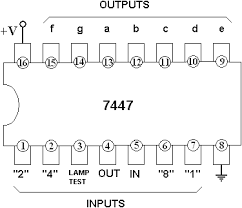
\includegraphics[width=0.5\linewidth]{bcd.png}}
  \hspace{\hfill}
  {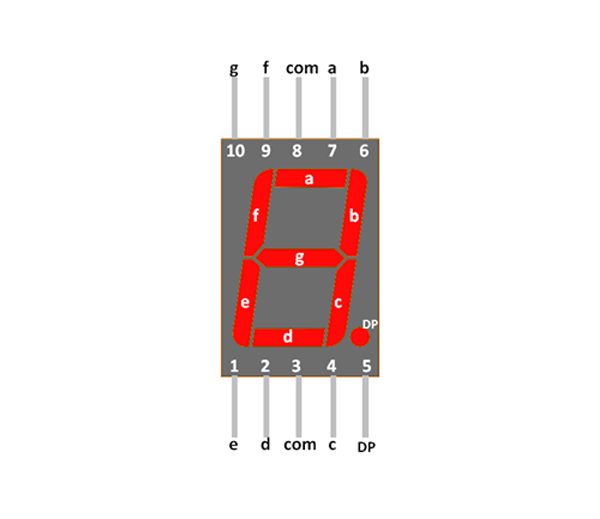
\includegraphics[width=0.5\linewidth]{7seg.png}}
\end{figure}
\section*{Results}
The working of the circuit is demonstrated in the video given in our github repository:
\newline
\href{}{\textcolor{blue}{Circuit Demonstration Video}}
\end{document}
